
\section{2 Dimensional Analysis}
This section will discuss the trend and effect of various undertray variables in 2 dimensions. The variables tested consist of inlet and diffuser angle where the optimised value will be used as a preliminary variable in a 3-dimensional undertray design. The 2D analysis will consist of an Enclosed flow analysis which use the Venturi-tube like geometry to simulate the flow of the undertray, and open-flow analysis used the bluff body to simulate the flow behaviour as well the interaction between the undertray and the bluff body. 

\subsection{2D Enclosed Flow}
2D Enclosed flow analysis serves a purpose in creating a fundamental understanding of the undertray flow physics. The diffuser and inlet angle was chosen to be the main variables which fundamentally known to affect the undertray's performance. It is so-called 'Enclosed' due to its geometry shaped like a half venturi meter that cap the flow analysis to only the lower part of the undertray without considering any surrounding flow ahead and behind the car itself. 

\subsubsection{Geometry and Mesh Generation}
\noindent The general geometry of this analysis is illustrated in figure \ref{fig:2D_EN_Geom} below. A realistic preliminary dimension was chosen to obtain a general picture of the undertray shape in 2D. The geometry represents the underside of the car, which consist of the undertray (top-wall), moving-floor (bottom-wall), velocity-inlet (left), and outlet (right). At this stage, the car's length was generalised to be 2000 mm, with 200 mm inlet and 600 mm diffuser horizontal length. Gap clearance (the minimum distance between the undertray and the floor) has been chosen to be 30 mm, which comply with the minimum gap clearance distance rules of FSUK. The undertray's geometries were generated in 2 varying variables; the first form is the increase of diffuser angle from 10 to 20 degrees in the increments of 2 degrees and accompanied with 10 degrees inlet angle for every geometry. The second form is the increase of inlet angle from 10 to 20 degrees in the increments of 2 degrees and accompanied with 10 degrees diffuser angle for every geometry. This format allows a preliminary development in understanding the effect of both undertray's outlet and inlet angle in an isolated flow-field. 

\begin{figure}[!ht]
    \centering
    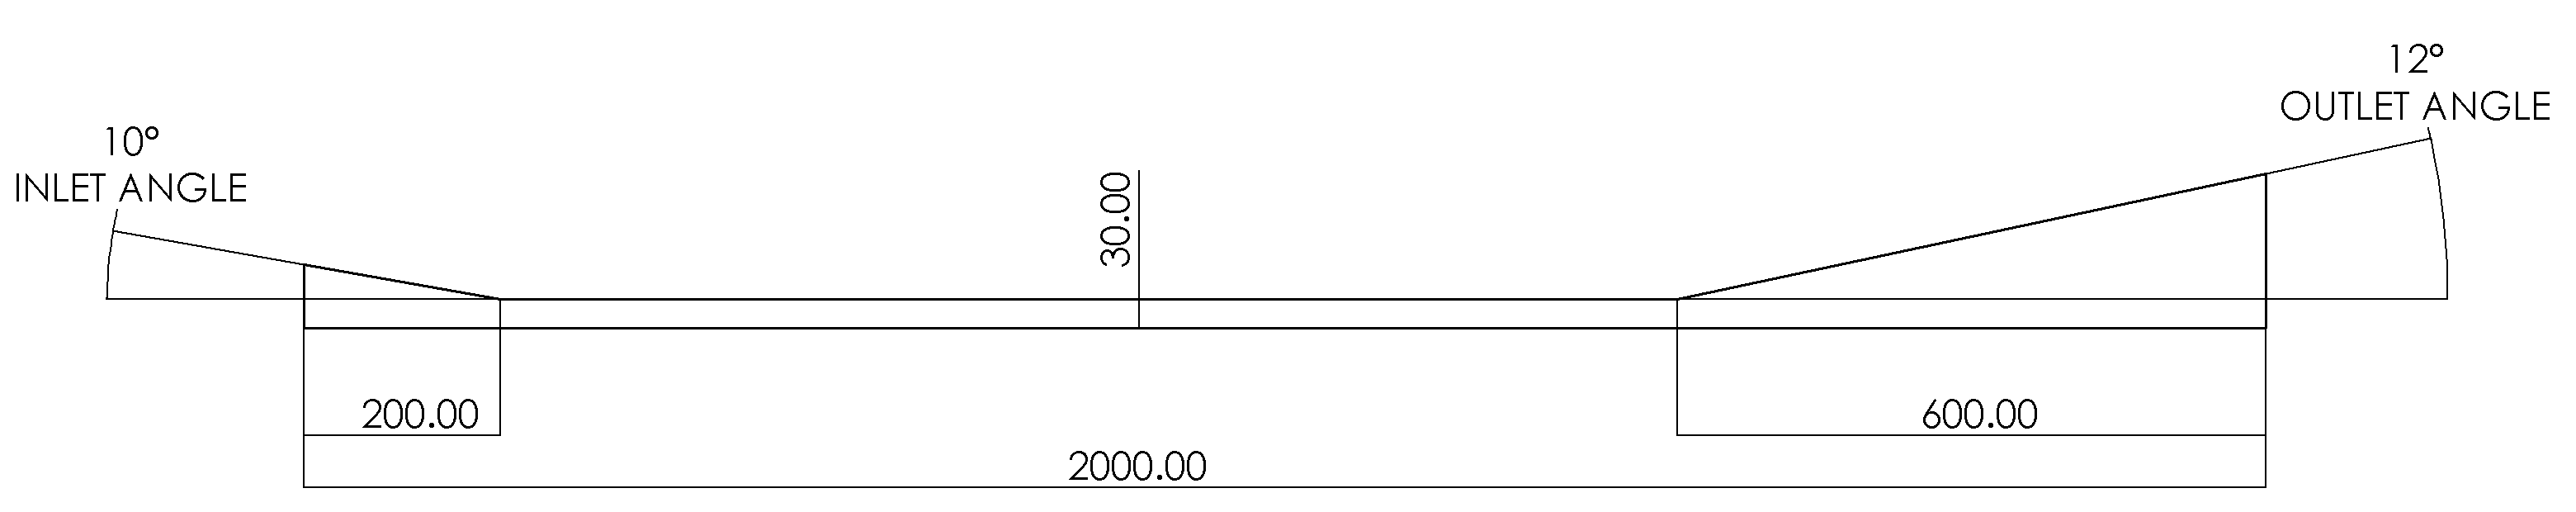
\includegraphics[scale=0.18]{Figures/2D_EN/2D_EN_D.PNG}
    \caption{2D Enclosed Geometry}
    \label{fig:2D_EN_Geom}
\end{figure}
  
\noindent A structured quadrilateral mesh was generated, and the inflation layer was initialised on the underside of the undertray. Twenty layers of inflation with the value of y$^+$ = 1 which gives the first layer distance of 2.24x$10^{-5}$ meters. Generally, the mesh element generated for each geometry in 2D Enclosed Flow analysis is around 20000 to 25000 elements depending on the variable. The mesh quality produced is considerably good with a skewness average of 3.67x$10^{-2}$ and an aspect ratio average of 31, which slightly above the range of recommendation \cite{Lanfrit2005BestFLUENT}; however, the convergence criterion is still met. Figure \ref{fig:2D_EN_MESH} in appendix A shows a mesh generated from one of the 2D enclosed geometries with inflation layer details.

\subsubsection{Results \& Discussion}
These analyses will be discussed based on how changes in outlet and inlet angle affected the downforce (negative lift) and drag of the undertray. Figure \ref{fig:2D_EN_result} depicts plotted lift and drag of the simulations for both variables and turbulence models. Figure \ref{fig:2D_EN_result} left shows the trend of undertray's lift and drag with changes of diffuser angle variable and the inlet angle variable on the right. 

\noindent k-epsilon and k-omega turbulence model were employed in this analysis as recommended\cite{} and discussed in section(). As shown in figure \ref{fig:2D_EN_result} below, a similar trend emerged for both turbulence model. There is no significant difference in both numerical method; however,  some anomalies occurred in some of the results. For instance, both k-omega lift at 16-degree diffuser and inlet angle, and the k-omega drag at 20-degree inlet angle are considered to be a little higher than the trend pattern. Nonetheless, pattern from both variables are clear and can be used as a preliminary understanding of the undertray.

\begin{figure}[!ht]
  \noindent
  \makebox[\textwidth]{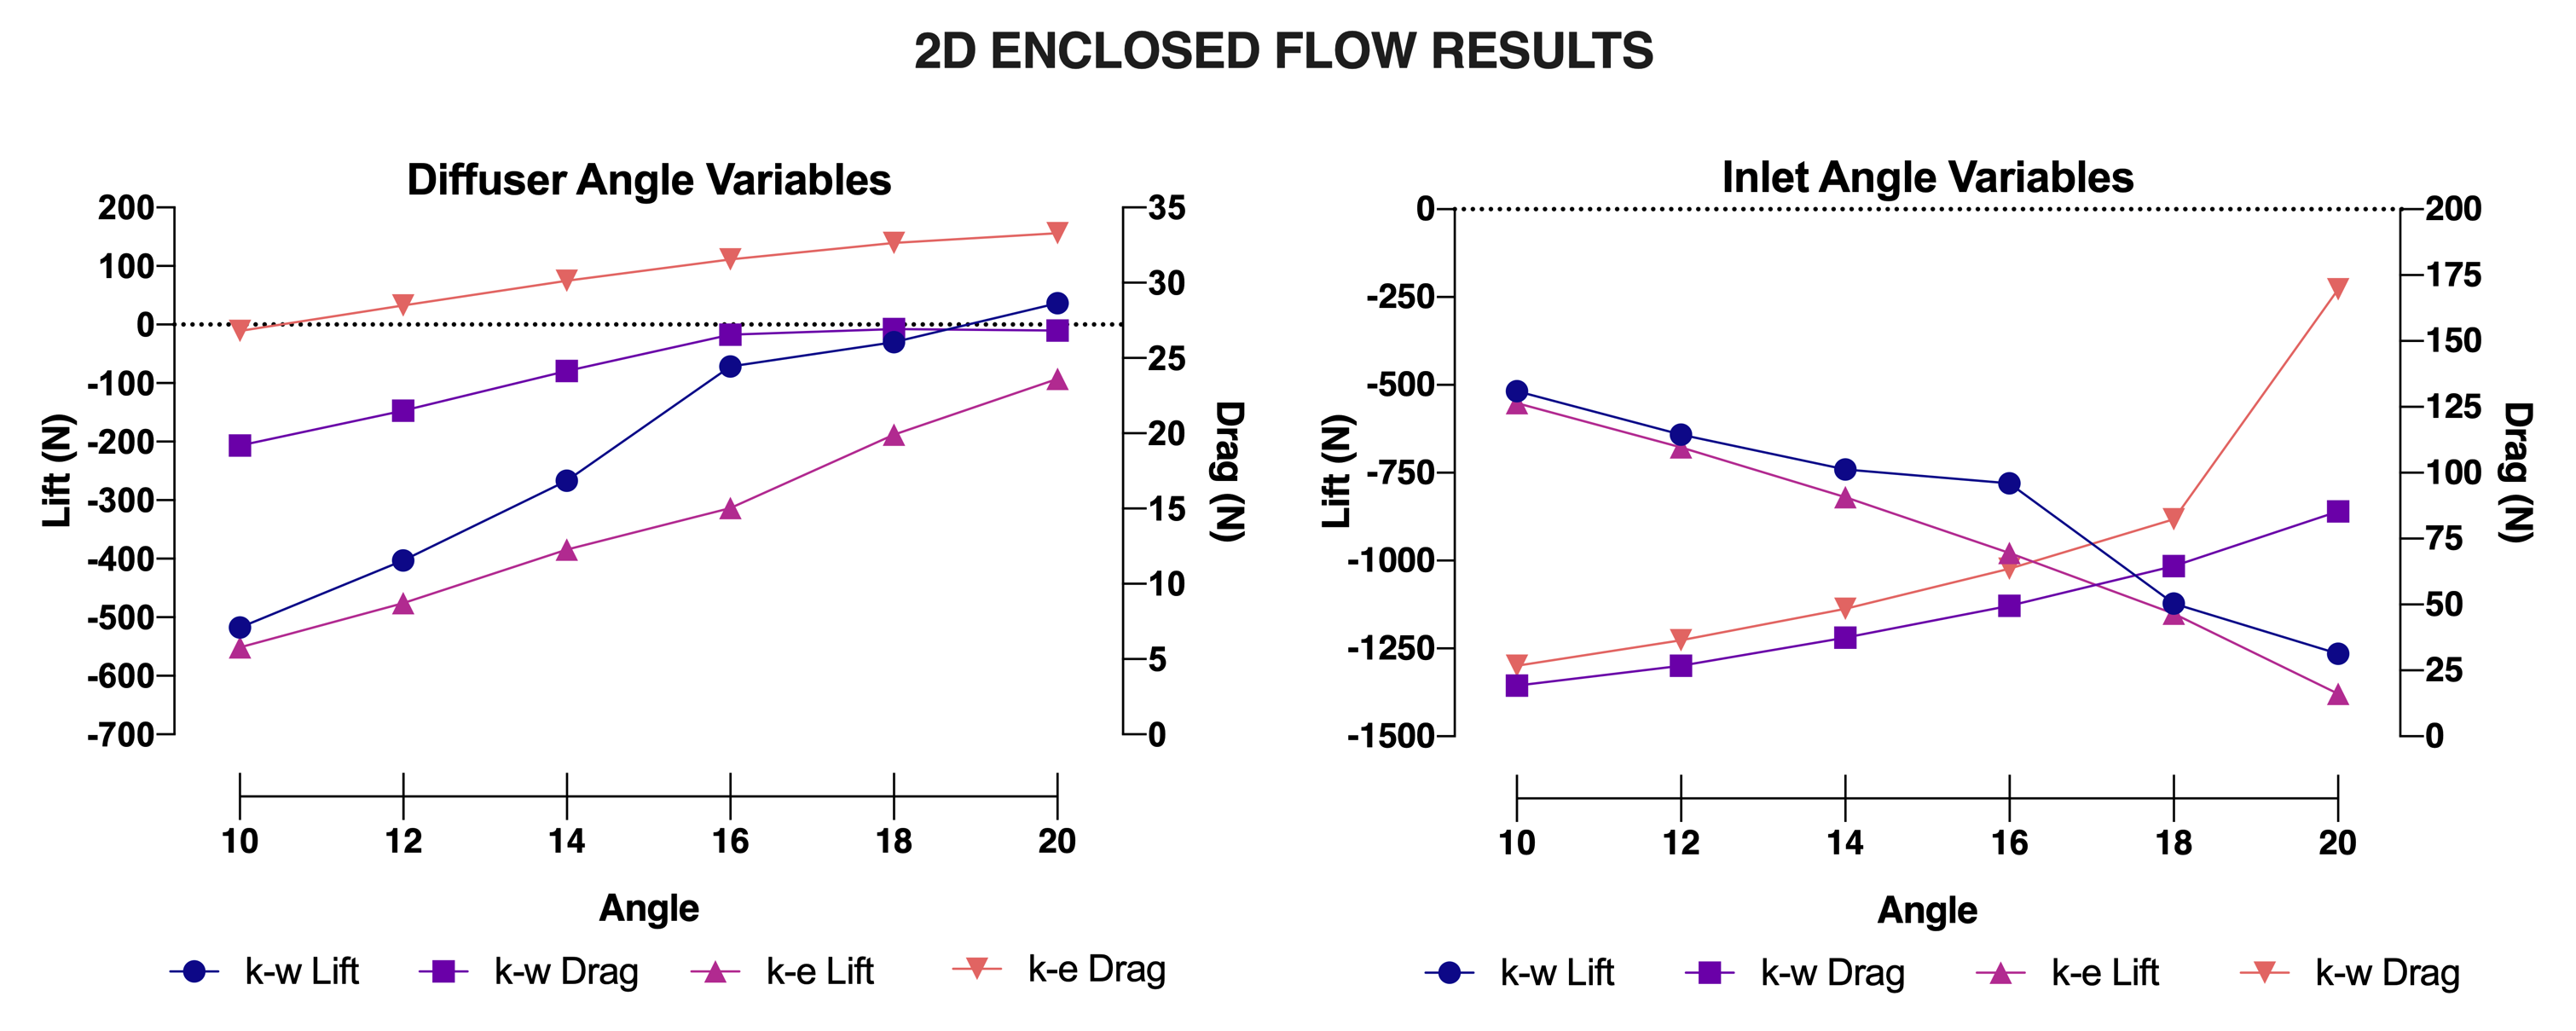
\includegraphics[scale=0.65]{Figures/2D_EN/2D_EN.png}}
  \caption{Lift and drag plot of 2D Enclosed flow analysis trend for both diffuser (left) and inlet (right) angle variables. }
  \label{fig:2D_EN_result}
\end{figure}

\noindent The main goal of a diffuser is to slowly expand the accelerated flow from the undertray's throat, which acts as the pressure and flow recovery system of an undertray. An efficient diffuser allows slow pressure recovery, which indicated by the flow attachment throughout the diffuser's wall. However, the diffuser angle variable plot on \textbf{figure \ref{fig:2D_EN_result}} left shows a linear degradation in the undertray's performance. The plot trend shows an increase in diffuser angle that directly proportional to the undertray's lift and drag; this is generally due to early flow separation on the transition region between the undertray's throat and diffuser region. 

\noindent Sharp corner and high velocity are the main issues that detach the flow early and create a sudden pressure change. Figure \ref{fig:2D_EN_streamline_compare} shows the velocity streamline from both 10 degree and 20 degree diffuser angle. The figure shows a similar separation point of the streamline when the flow enters the diffuser region; this phenomenon is more obvious on the larger diffuser angle (fig \ref{fig:2D_EN_streamline_compare} (right)) as a low-pressure region formed, which indicated in dark blue colour. Linear increases in drag are explained by the low-pressure region formed on the diffuser area, which acts as a vacuum that pulls the undertray contrary to its direction.  

\begin{figure}[!ht]
    \centering
    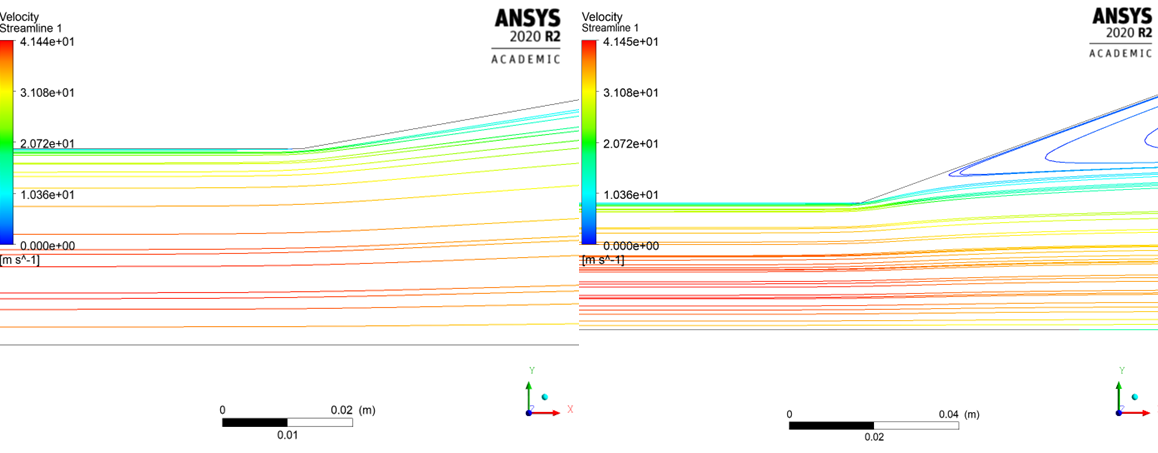
\includegraphics[height= 6cm]{Figures/2D_EN/2D_EN_Streamline_compare.PNG}
    \caption{Undertray's velocity streamline for 10 degree (left) and 20 degree (right) diffuser angle.}
    \label{fig:2D_EN_streamline_compare}
\end{figure}

\noindent From \textbf{figure \ref{fig:wall_shear_plot_2D_EN} left} in \textbf{Appendix A} ,  it can be observed that flow detachment occurred at an identical point of the undertray at any given diffuser angle, which indicated by a similar pattern of the second peak on the graph. Moreover,  flow detachment also occurred due to the adverse pressure gradient, which is indicated on the second lower peak on the static pressure plot in figure \ref{fig:pressure_plot_2D_EN} \textbf{Appendix A}.

\noindent On the other hand, the inlet angle variable has a contrary result to the previous variable. \textbf{Figure \ref{fig:2D_EN_result}} right shows that the lift is inversely proportional to the drag as the inlet angle increases.  As the cross-section area on the inlet nozzle converging, the flow is forced to convert the pressure energy into kinetic energy indicated by the increase in its velocity, which then drops the pressure in the undertray's throat. This condition creates a lower pressure region on the undertray's throat, hence increasing the downforce. This phenomenon obeys the Bernoulli equation \textbf{ (equation \ref{eq:bernoulli})} where pressure and cross-sectional area is inversely proportional to the flow's velocity, assuming the flow in the inlet region are steady and incompressible.  Elevation in inlet angle also provides a more tangential surface to be imposed by the incoming flow; this creates higher shear stress on the inlet wall and increases the overall drag. This condition also indicated on the first peak of the wall shear on figure \ref{fig:wall_shear_plot_2D_EN} left, which shows a significant increase in shear stress at the corner between the inlet and throat region.

\noindent Further analysis of wall shear stress \textbf{(figure \ref{fig:wall_shear_plot_2D_EN} right)} and static pressure \textbf{(figure \ref{fig:pressure_plot_2D_EN} right)} plot for inlet angle variables in \textbf{Appendix A} shows a general increase in shear stress with inlet angle elevation accompanied by the overall pressure drop as the angle increases. This explains the increase in total downforce with the elevation of the inlet angle.

%%%%%%%%%%%%%%%%%%%%%%%%%%%%%
%%% 2D OPEN FLOW ANALYSIS %%%
%%%%%%%%%%%%%%%%%%%%%%%%%%%%%


\subsection{2D Open-Flow}
The previous analysis provides a fundamental understanding of how changes in inlet and diffuser angle may affect its overall performance and solely focus on the internal flow of the undertray without taking account of the flow surrounding it. This section will be an extension of the previous analysis to understand the effect of a similar variable with an additional bluff body added to the geometry. 

\subsubsection{Geometry and Mesh Generation}
This section will utilise multiple types of bluff bodies to simulate the flow behaviour around the body and how it will affect an undertray's general performance. Four different geometries were built on a generative decision which each serve its own purpose in this analysis. A rough calculation of the QFR car's length was too initiated. Geometry 1 \& 2 has 2.6 meters of undertray length with a similar inlet and diffuser configuration as previous analysis. However, Geometry 3 has a slightly different undertray configuration, with 2.85 meters of length, 1-meter smooth rounded diffuser, and 0.25 meters of inlet angle. Worth noting that the code 'A' stands for 'analysis', which corresponds to the type of geometry used in the discussions and figures.

\begin{figure}[!ht]
    \centering
    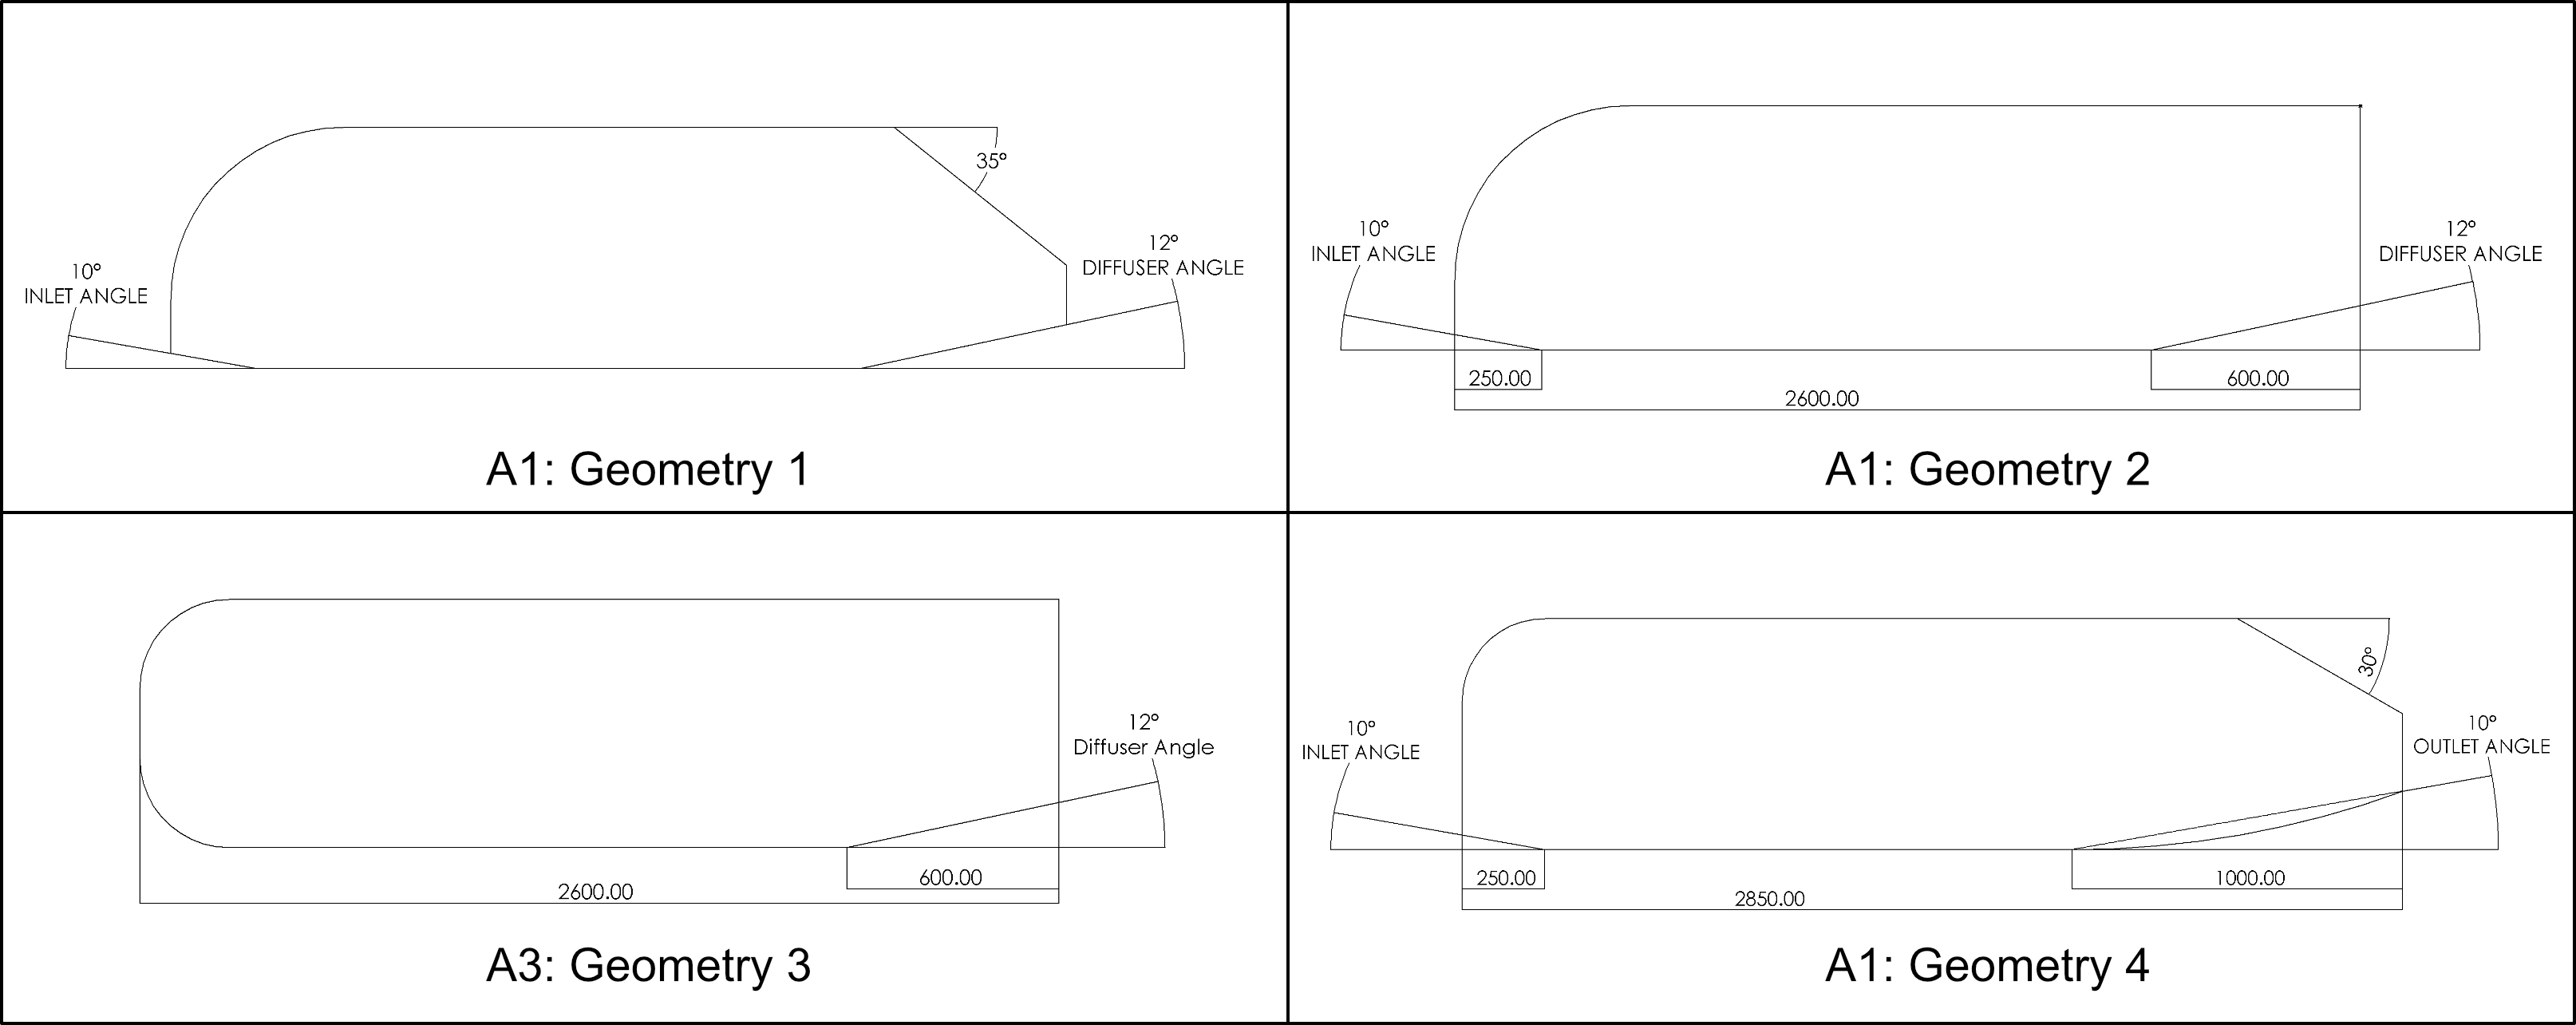
\includegraphics[scale = 0.5]{Figures/2D_OF/2D_OF_GEOM.png}
    \caption{Four geometries generated for 2D open-flow analysis.}
    \label{fig:2D_OF_GEOM}
\end{figure}

\noindent The geometry can be grouped into two categories. The first category consists of A1, A2, which focuses on how the geometry of the bluff body sculpts the surrounding flow and affects the overall performance of the undertray. First geometry acts as the baseline model with a 35-degree slant angle at the rear body to simulate the flow separation that also occurs at the rear of the QFR car. Similar to geometry 1, the second geometry has a similar dimension without inlet variable and the slant angle to simulate an immediate separation at the rear body.

\noindent Second category consists of geometry 3, which is the regeneration due to previous analysis. This geometry used a curved diffuser configuration where one end is tangential to the throat. A construction line was made between two points of the diffuser as an angle reference point from the horizontal axis. In diffuser variable analysis, a rounded inlet such as geometry three without any elevation was used. The purpose of such rounded inlet and diffuser was initially surmised to allow smooth intake and slows flow separation in the diffuser region due to the sharp transition from previous analyses. A Slant angle of 30 degrees was also decided to be utilised to provide geometric similarity to the QFR car.

\noindent A hybrid mesh was generated for this analysis. This consist of unstructured triangular and quadrilateral mesh (or inflation) near the bluff body and the floor to identify the effect of boundary layer interaction between the undertray and floor wall.  Detailed graphics of 2D open-flow mesh can be seen on \textbf{figure \ref{fig:2D_OF_MESH}} in \textbf{Appendix B}.
%add details average of the mesh quality criterion (mesh number, AR, skewness, quality)

\subsubsection{Results \& Discussion}

\noindent A 2D computational simulations have been done, and the results shown will be based on the downforce and drag of the entire bluff body. Analysis 1 and 2 have a geometric similarity apart from the slant angle. The first part of the discussion will focus on how the slant angle affects the rear flow and its impacts on the undertray's performance. Figure \ref{fig:2D_OF_A12_results} below depicts the variations in trend in downforce (left) for both diffuser and inlet angle. The variations of lift and drag due to the inlet angle is also shown in figure \ref{fig:2D_OF_A12_results} (right).

\begin{figure}[!ht]
    \centering
    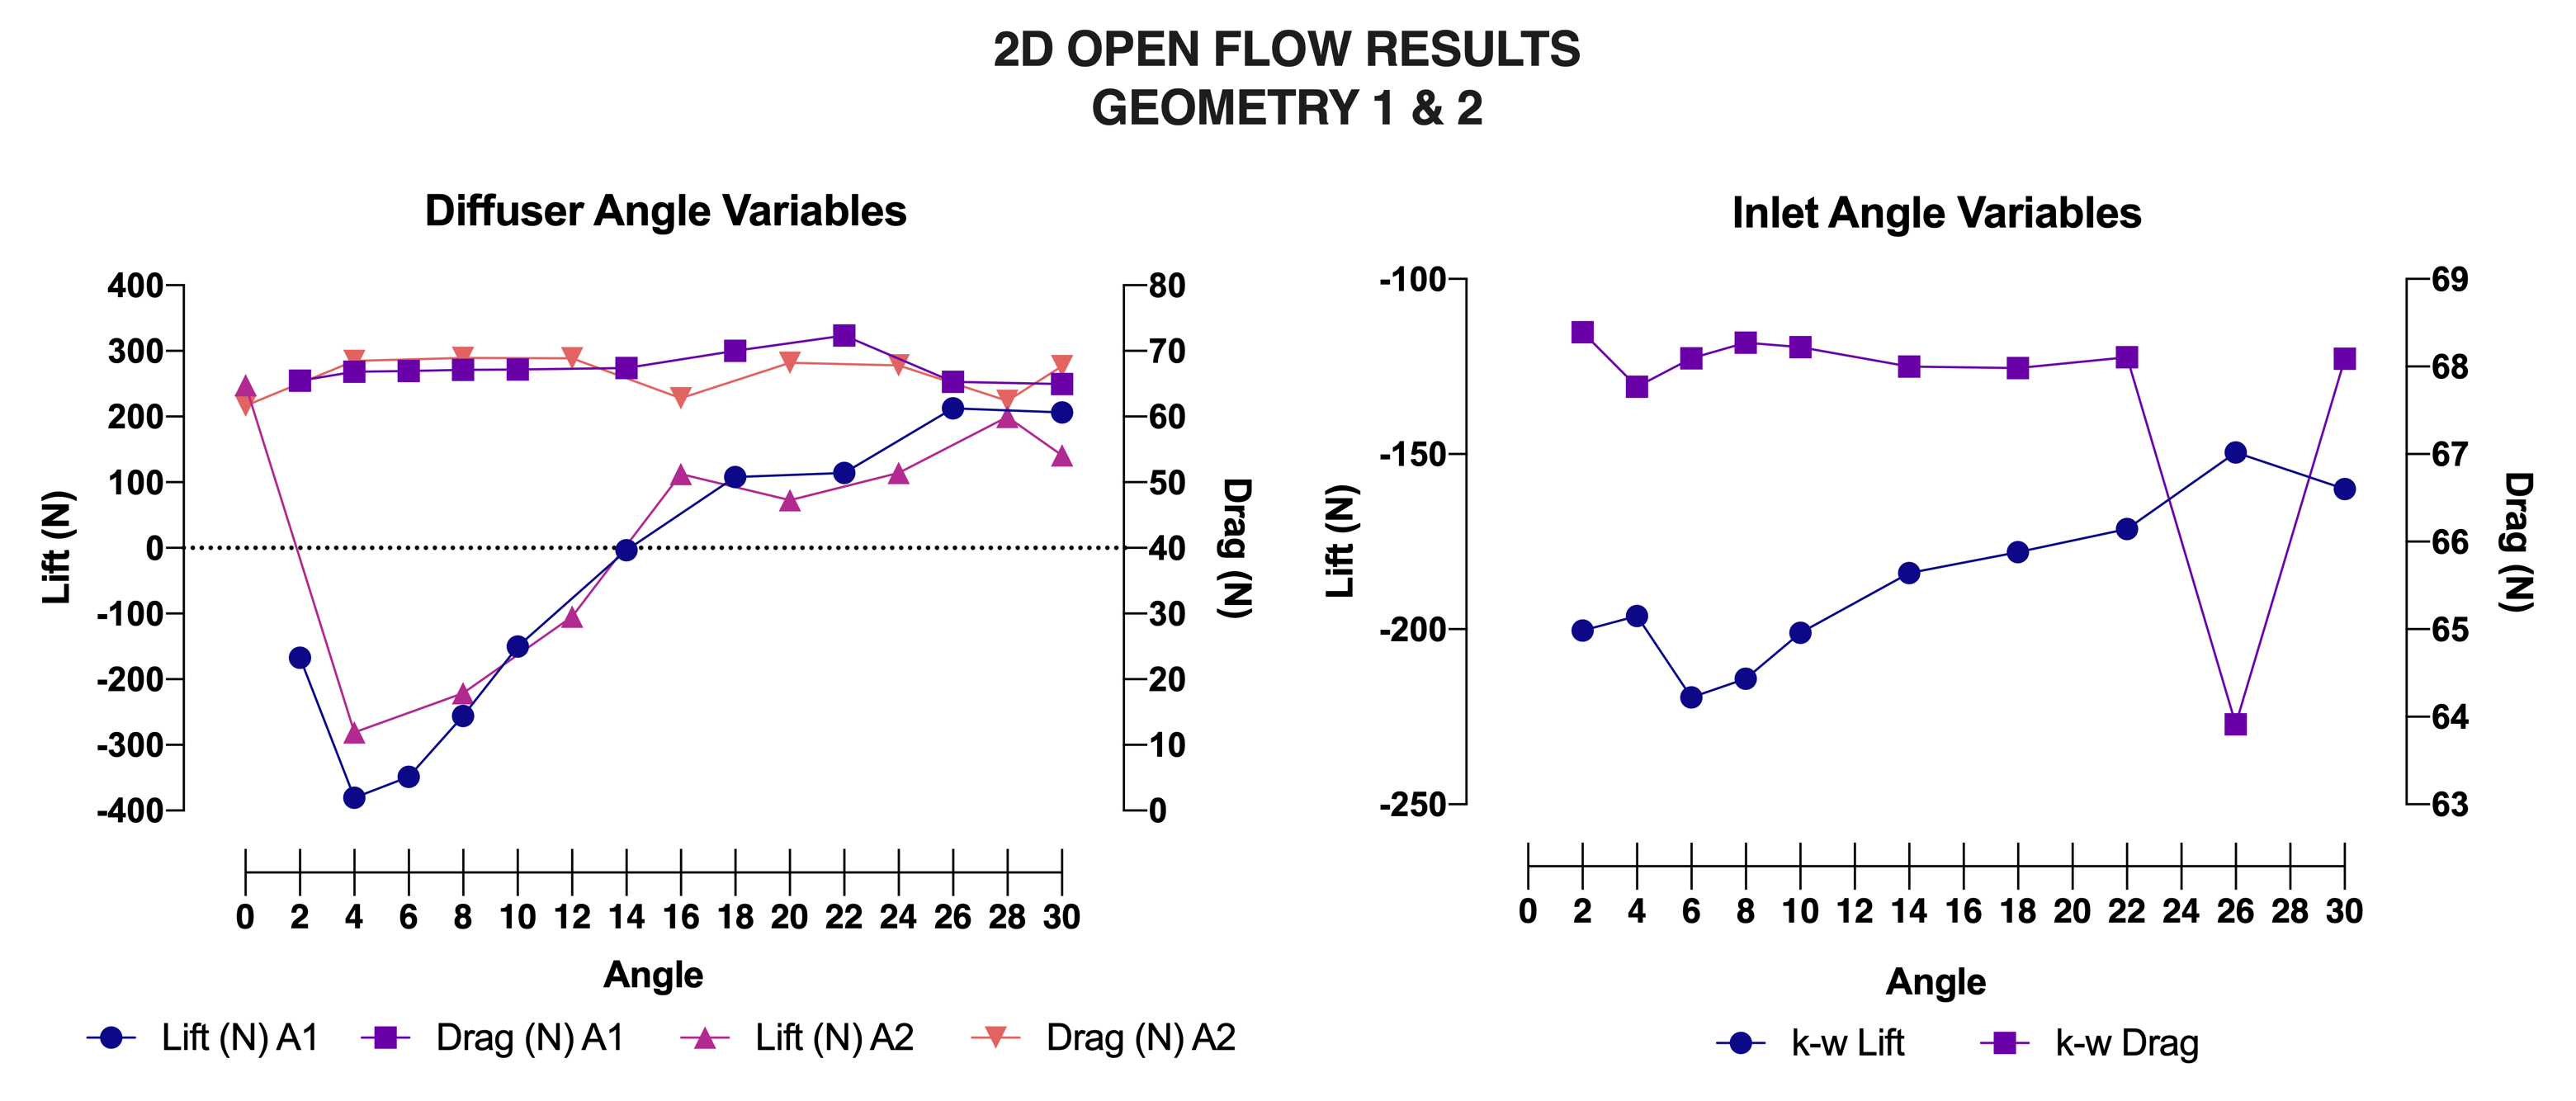
\includegraphics[scale = 0.6]{Figures/Graph/2D_OF_A1-2.png}
    \caption{Lift and drag variation vs inlet and diffuser angle variable on geometry 1 and 2. }
    \label{fig:2D_OF_A12_results}
\end{figure}

\noindent The 2D enclosed analysis has a range of 10 to 20 for inlet and diffuser angle, and this analysis was conducted to further investigate the flow behaviour in a larger range of elevation. In figure \ref{fig:2D_OF_A12_results} left, lift and drag trend due to the diffuser angle elevation can be observed. A significant drop in lift occurred for both A1 and A3 from 0 to 4 degrees. A small angle in the diffuser allows the flow to stay attached to the diffuser wall, allowing slower expansion in pressure that increase the overall downforce. This can be indicated on the velocity contour in figure \ref{fig:2D_OF_10_4_Contour_compare} (left) below, where the formation of adverse pressure gradient on the diffuser  (indicated in blue region) is delayed at 4 degrees compared to 10 degrees where separation occurred around the transition region. Further analysis in flow separation can be seen in figure \ref{fig:2D_OF_10_4_Contour_compare} (right)  that shows the comparison of wall shear and pressure along with the undertray for both geometry 1 and 2. 


\begin{figure}[!htb]
    \centering
    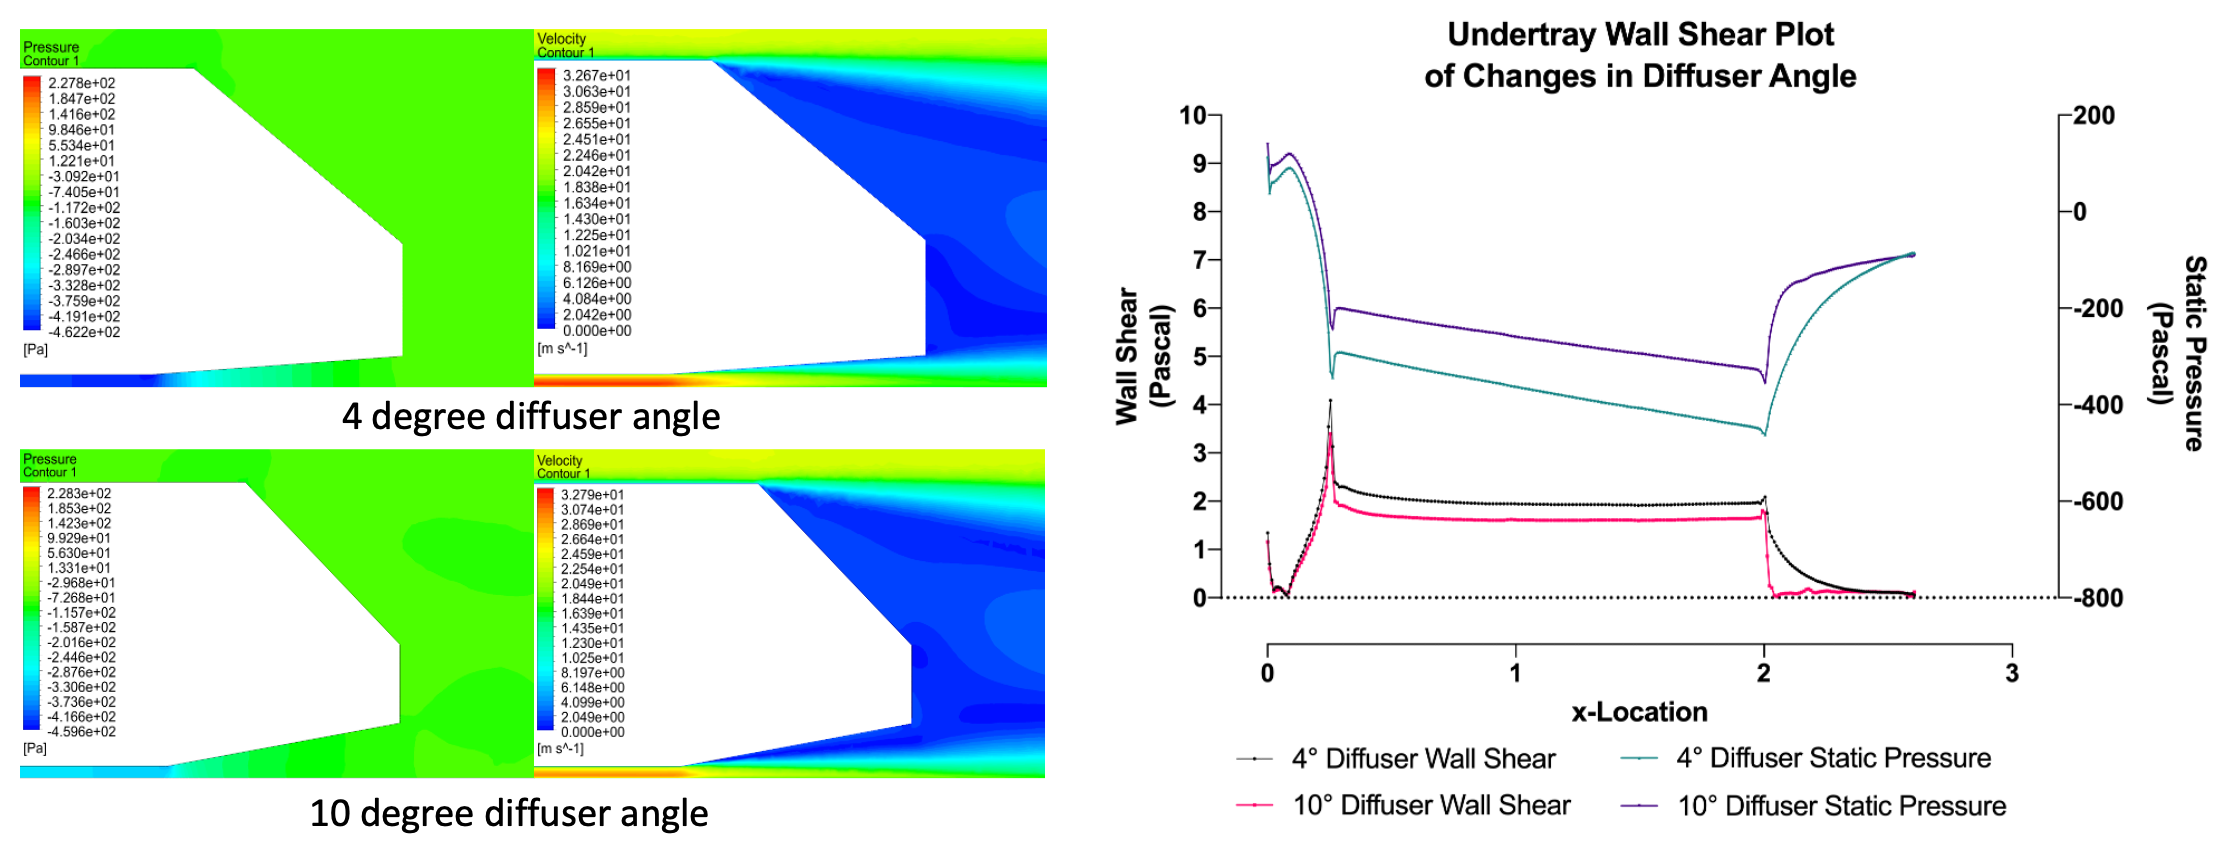
\includegraphics[scale=0.52]{Figures/2D_OF/10_4_O_COMPARE CONTOUR.PNG}
    \caption{Comparison of 4 and 10 degrees diffuser angle with regard to flow separation on the diffuser region }
    \label{fig:2D_OF_10_4_Contour_compare}
\end{figure}

\noindent Following the drop in lift at 4 degrees, degradation in downforce performance is indicated on the graph, representing the 2D enclosed lift analysis from 10 to 20 degrees. However, no significant drag changes and pattern emerged with the change of diffuser angle. From both analyses, the slant angle's presence deemed to not affect the overall lift and drag of bluff body on both geometries, which indicated by an identical lift and drag trend. It is shown in figure \ref{fig:2D_OF_A1_CONTOUR}, Appendix B, that flow separation occurred immediately at the slant angle, which indicates similar flow features at the rear compared to geometry 2 (\textbf{see figure \ref{fig:2D_OF_A2_CONTOUR}, Appendix B}). 

\noindent On the other hand, the inlet variable shows a contrary trend to 2D Enclosed flow, where the elevation of inlet angle is inversely proportional to the downforce. The flow imposed generate a stagnation point on the front body, which the point that separates the flow ahead to the top and the undertray. This occurrence slows the velocity flow that enters the inlet region, hence reduced the overall effectiveness of energy conversion. In comparison, the 2D enclosed flow has a perfect flow intake without any turbulence disturbance and variable velocity. As it enters the inlet angle of 22 degrees, the low-pressure region at intake is insignificant; however, this occurrence is clearer at the transition between the intake and throat indicated by the blue velocity streamline. This can be further observed on the inlet pressure plot on figure \ref{fig:2D_OF_A1_PLOT} Appendix B; it can be seen that there is pressure fluctuation for 6 and 10-degree angle. This indicates the early low-pressure region, as explained earlier. Moreover, at 22 degrees inlet elevation, an immediate pressure drop is indicated by the plot at the transition corner between the inlet and throat region. Moreover,  It can be observed that immediate streamline on figure \ref{fig:A1_Contour_inlet_compare} redirection cause a low-pressure gradient which indicated by the empty velocity streamline region 

\begin{figure}[!hb]
   \noindent\makebox[\textwidth]{
   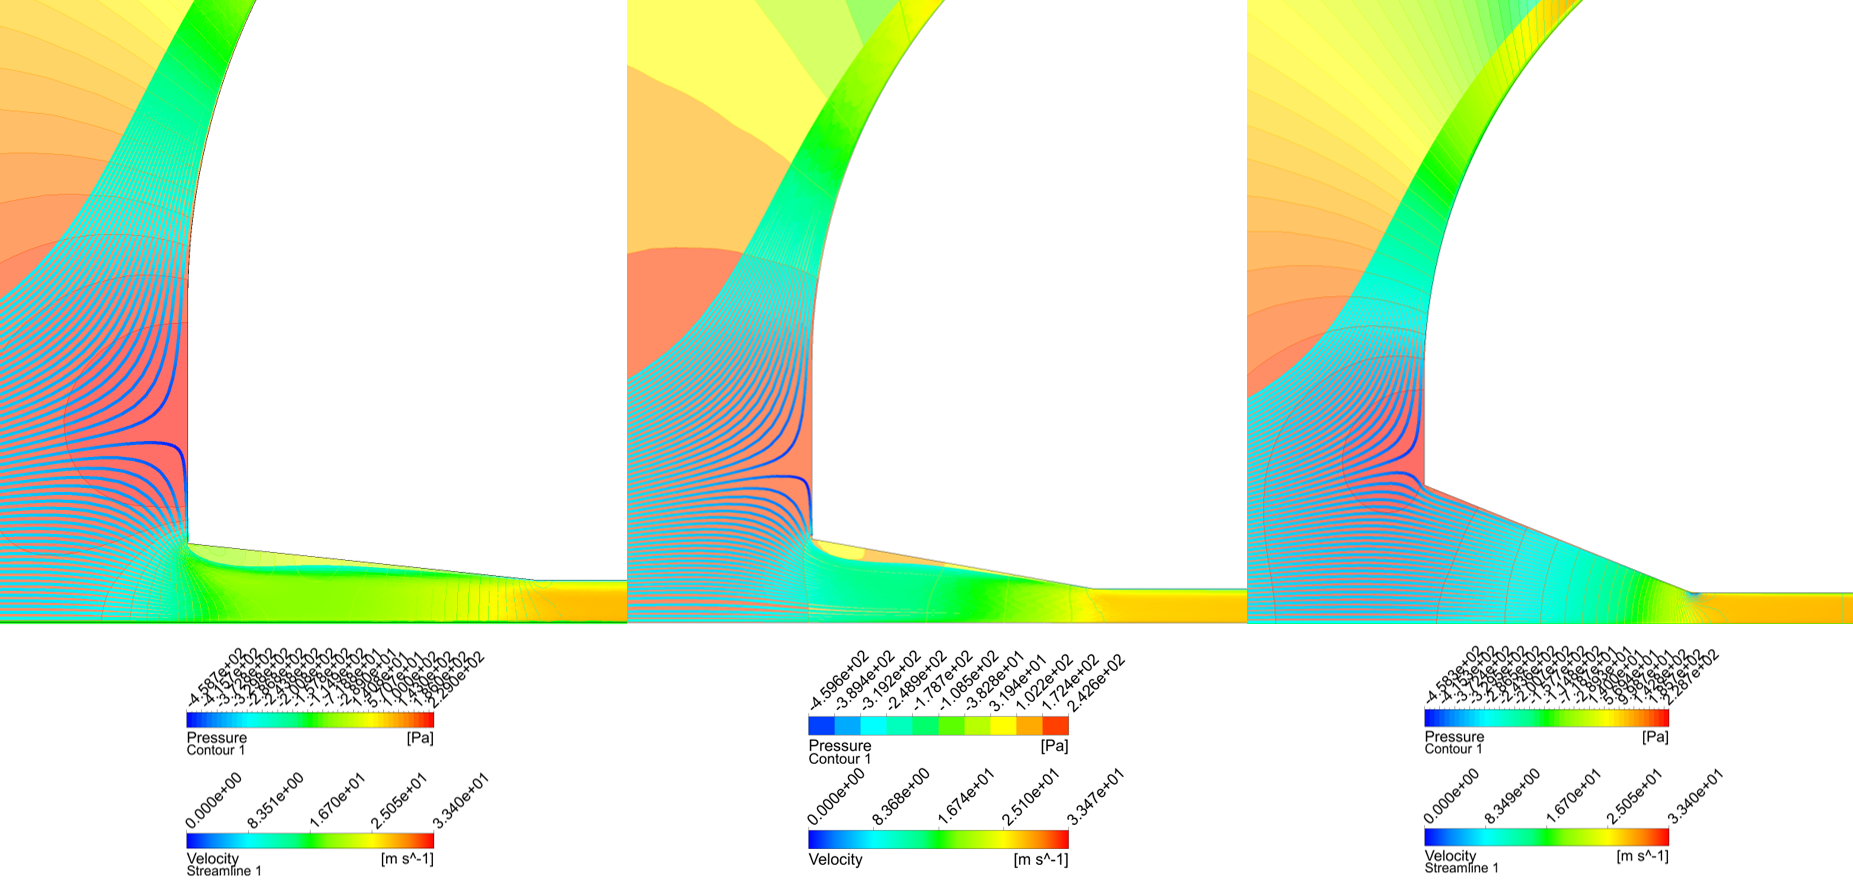
\includegraphics[width=0.8\textwidth]{Figures/2D_OF/2D_OF_A1_CONTOUR_INLET_COMPARE.png}}
   \caption{Comparison of velocity streamline and pressure contour of 6 (left), 10 (middle), and 22(right) degrees inlet angle. }
   \label{fig:A1_Contour_inlet_compare}
\end{figure}

\noindent It was observed that sharp corner might increase the possibility of early separation at some variable and location. Therefore, geometry 3 was fabricated to overcome these problems and investigate further similar variables. Figure \ref{fig:2D_OF_A4_results} below depicts the plot of variation in lift and drag vs inlet and diffuser angle of geometry 3.

\begin{figure}[!ht]
    \centering
    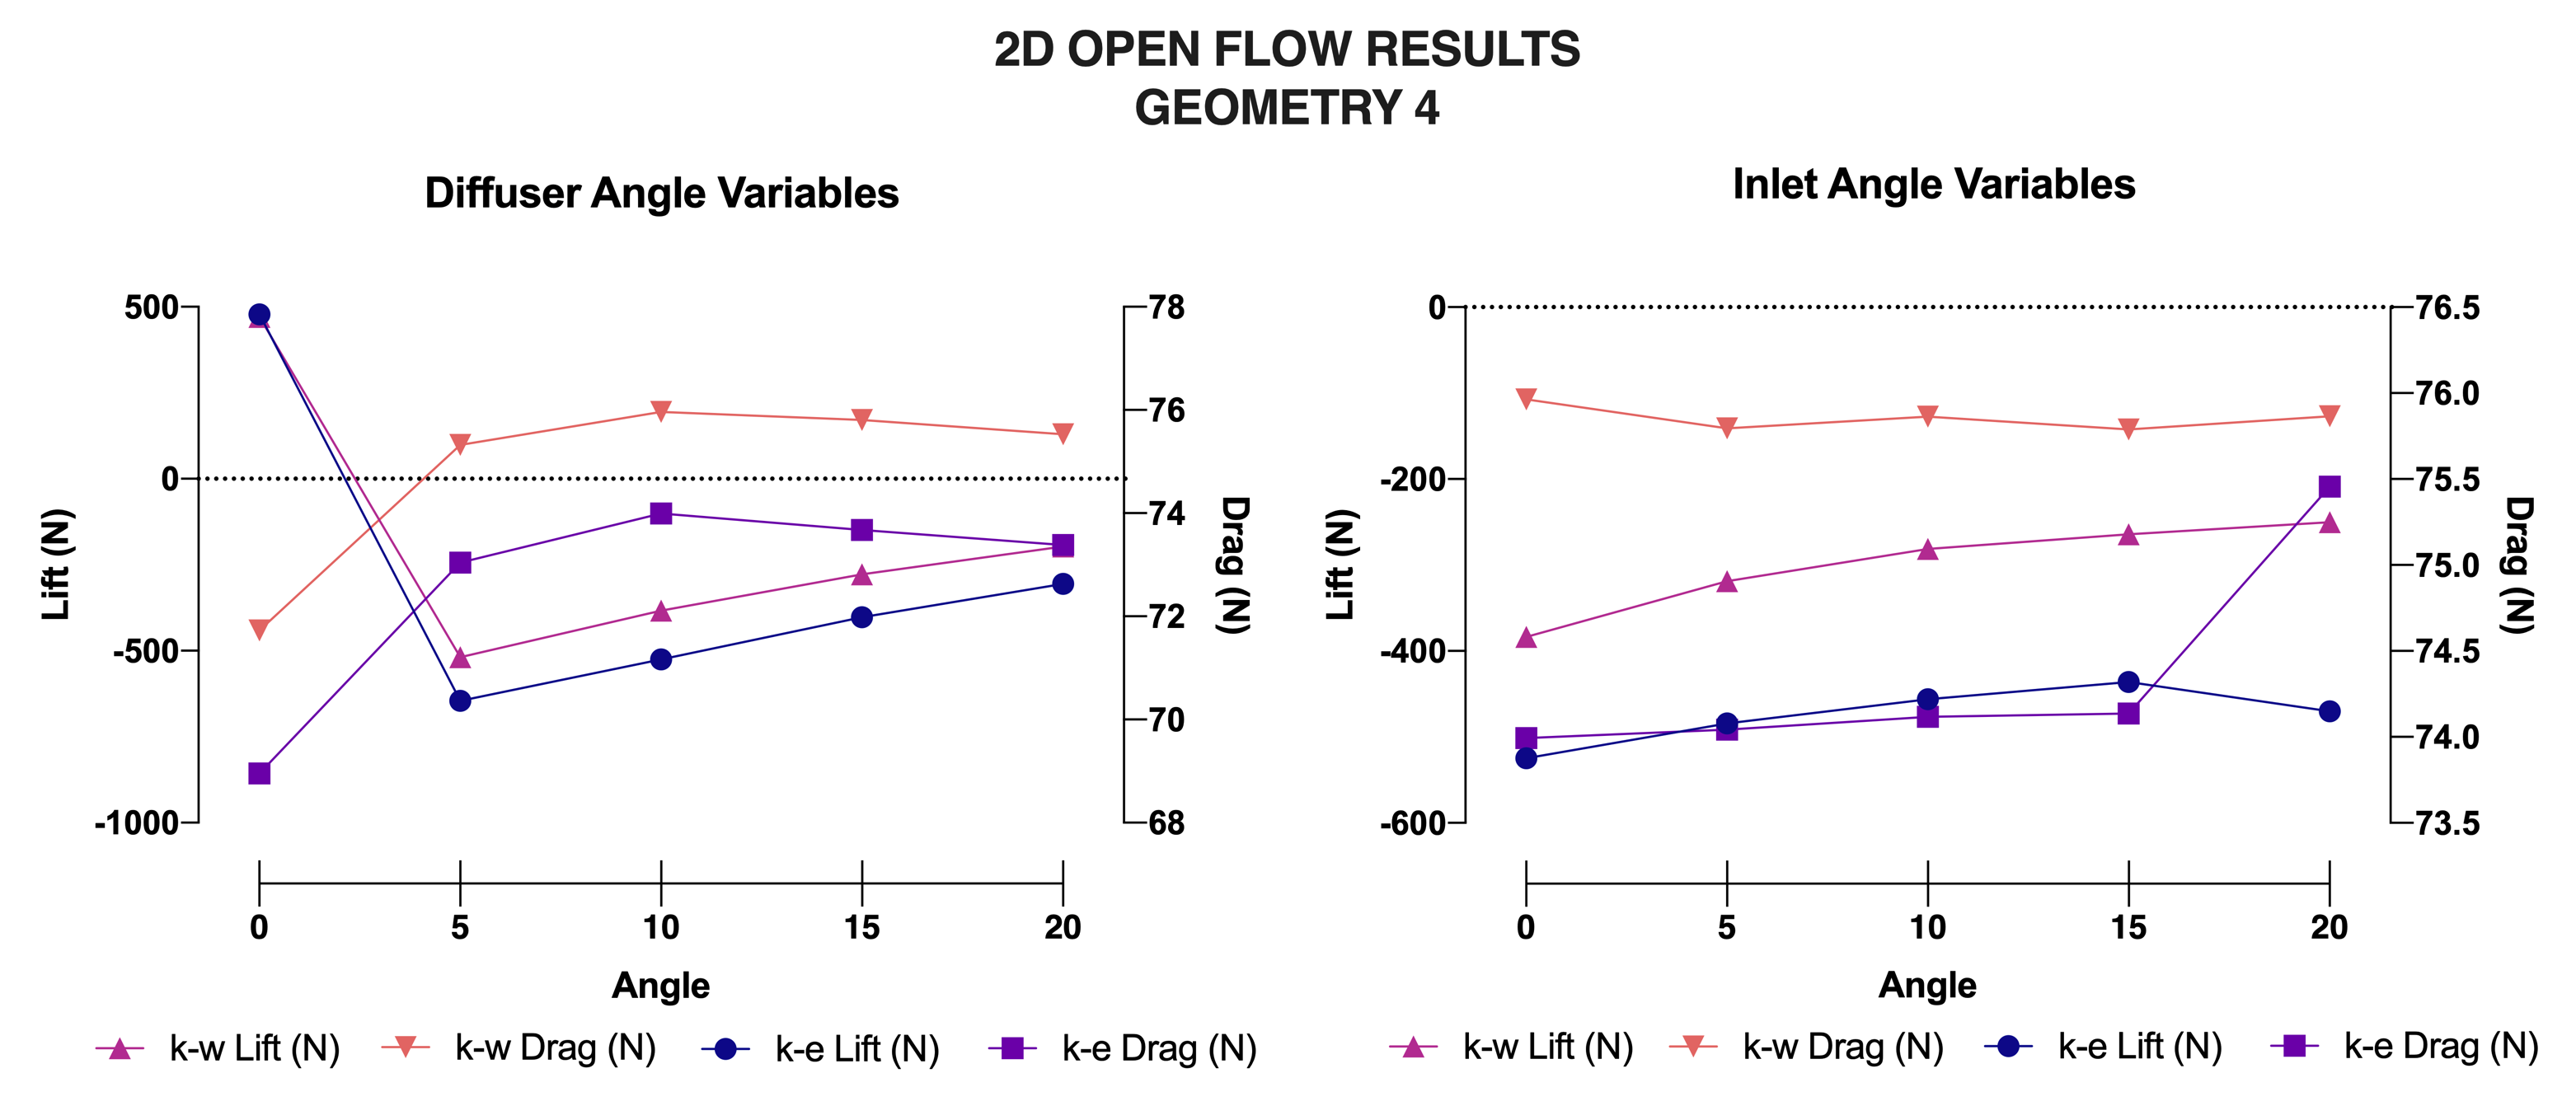
\includegraphics[scale=0.6]{Figures/Graph/2D_OF_A4.png}
    \caption{Lift and drag variation vs diffuser and inlet angle of geometry 3.}
    \label{fig:2D_OF_A4_results}
\end{figure}

\noindent Identical trend can be observed for lift vs diffuser angle for both geometry 2 and 3. A maximum downforce occurred at 5 degrees diffuser angle, followed by a linear decrease in downforce. From this analysis alone, a smooth and longer diffuser has shown to delay the flow separation, which increases the overall downforce. An increase in drag occurred up to its maximum point at 10 degrees then decrease subsequently; however, it is worth noting that the scale is small, which makes it insignificant. On the other hand, the inlet variable also shows a similar and clear trend due to the smoother intake. It can be seen that lift smoothly increase directly proportional to the inlet angle, and no fluctuations occurred, which surmised an effective flow intake where no disturbance of flow separation on the inlet region. Comparing all geometries analyses, it can be seen from figure \ref{fig:2D_OF_PLOT_COMPARE_ALL} below that the overall downforce of geometry 3 at any given angle after 5 degrees are generally lower, and the overall drag is too generally higher, however insignificant, compared to the rest of geometries.

\begin{figure}[htb!]
    \centering
    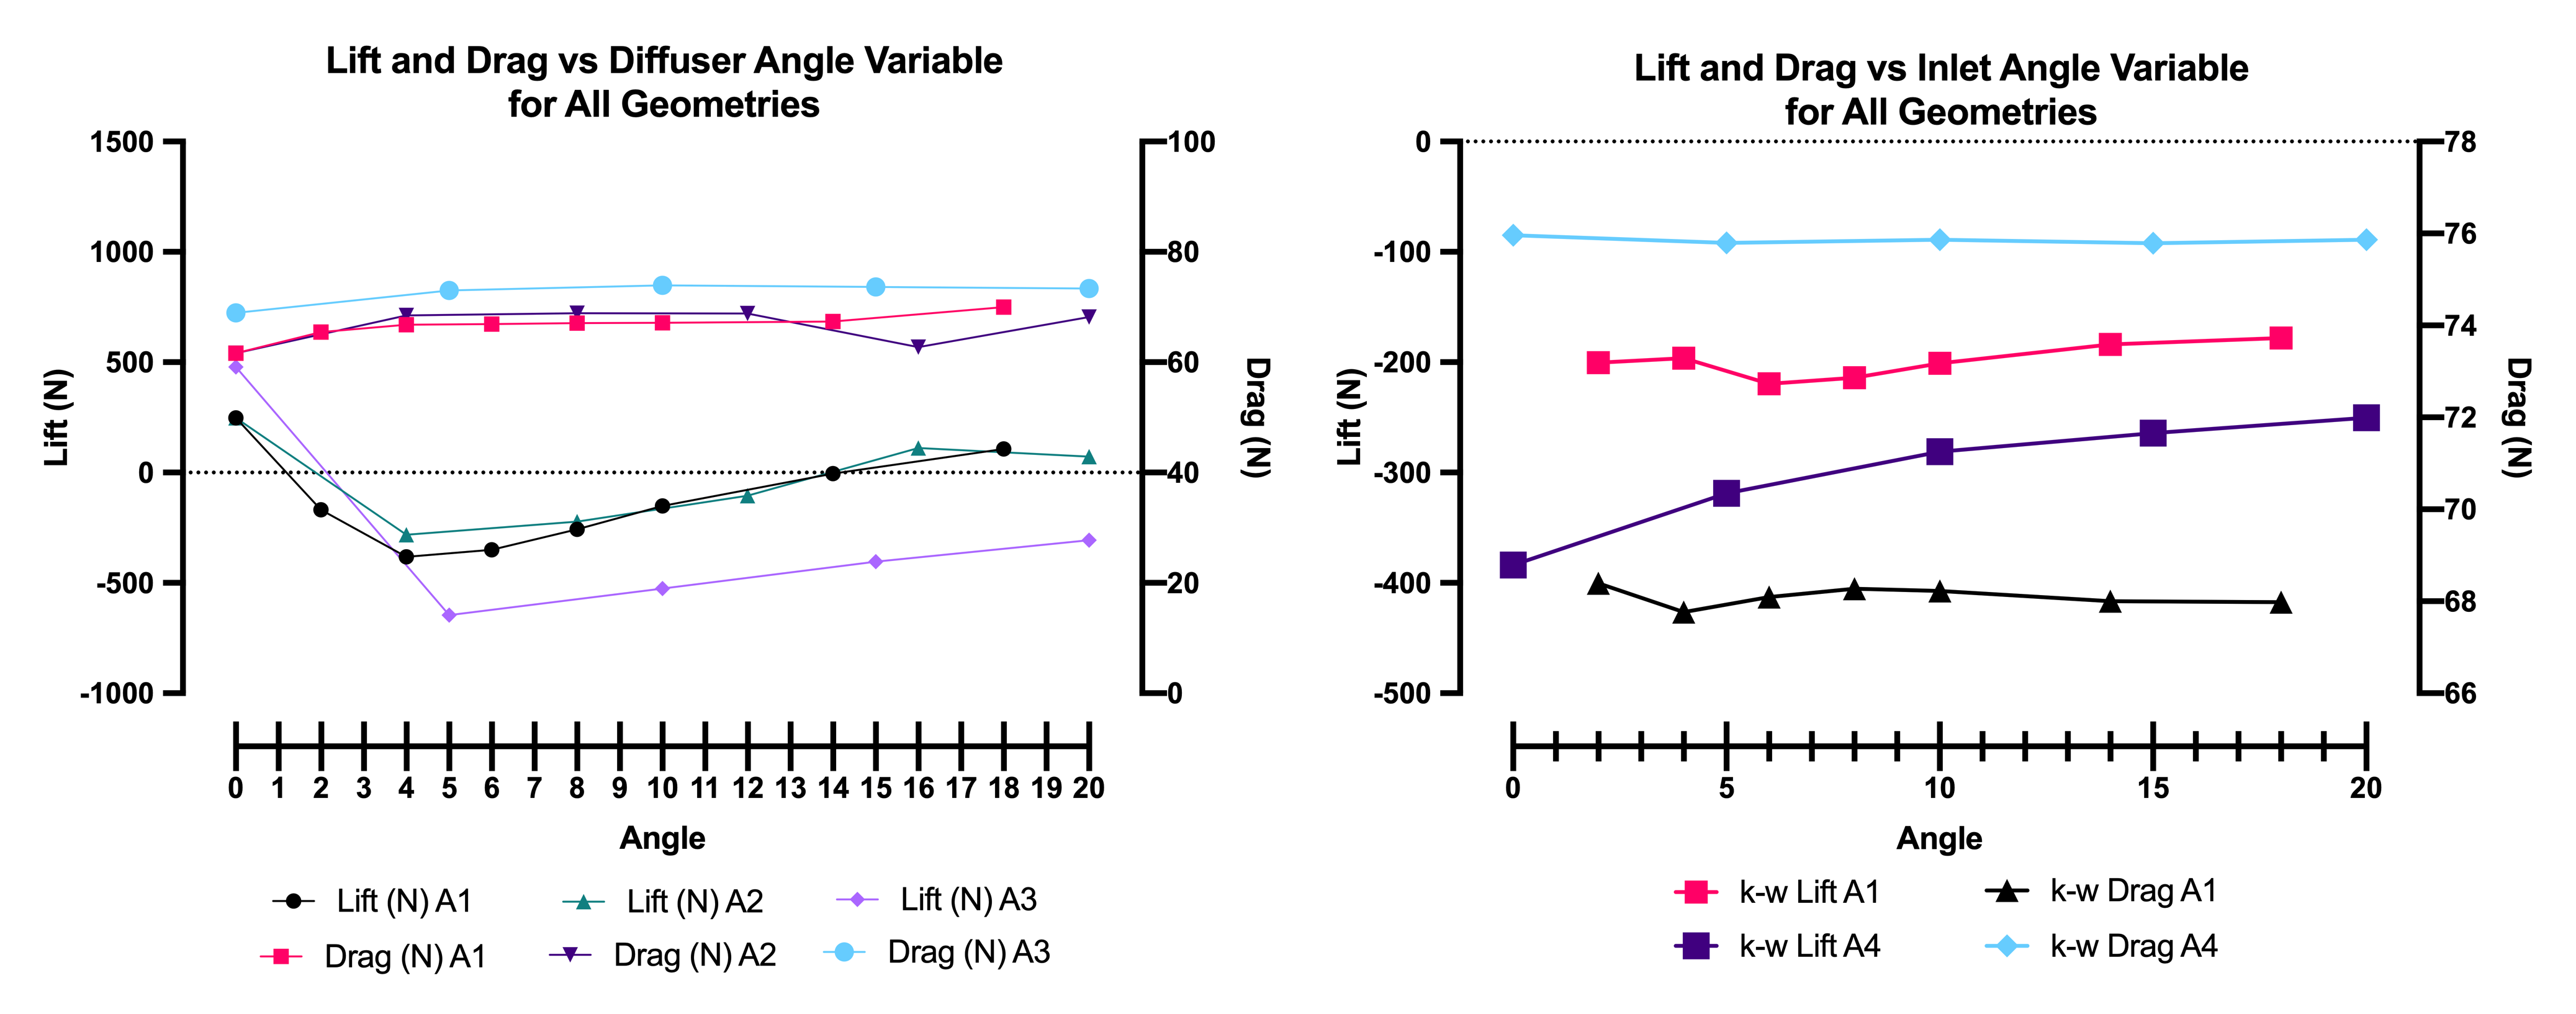
\includegraphics[scale=0.9]{Figures/2D_OF/2D_OF_PLOT_COMPARE_ALL.png}
    \caption{Lift and drag variation vs diffuser (left) and inlet (right) angle of all geometries.}
    \label{fig:2D_OF_PLOT_COMPARE_ALL}
\end{figure}

\noindent Similarly for the inlet angle variable, smoothed inlet angle allows a better flow intake which indicated by the overall downforce and drag of geometry 3 is higher than geometry 1. It is worth noting that 2D Open flow analyses indicate no significant drag changes for every variable; this is due to the significant drag produced by the flow separation at the rear bluff body itself, contrary to the 2D enclosed flow where drag only produced by the flow underneath. Hence, changes in undertray drag are inconsiderable compared to the bluff body drag.



